\begin{figure}[t]
\centering
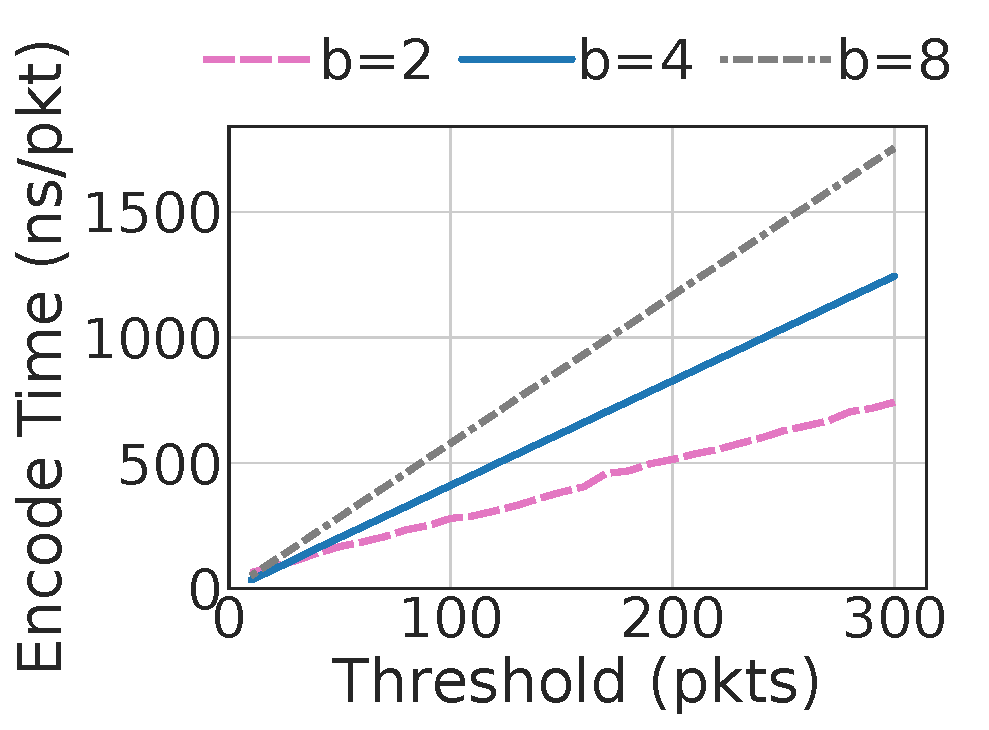
\includegraphics[width=0.37\linewidth,trim={3mm 0 7mm 0},clip]{quack/figures/fig2c_quack_threshold_vs_encode_time.pdf}
\caption{The encoding time of the power sum quACK scales linearly with the
 threshold $t$, and is generally higher for higher bit widths. If expect the
 typical threshold to be $<100$, then the typical encoding time is on the order
 of nanoseconds per packet. Average of 100
 trials, each trial is the average of 1000 packets.}
\label{fig:quack:psum-encode}
\end{figure}
